\documentclass[a4paper]{exam}

\usepackage{adjustbox}
\usepackage{geometry}
\usepackage{graphbox}
\usepackage{graphicx}
\usepackage{hyperref}
\usepackage{multirow}
\usepackage{tabularx}
\usepackage[table]{xcolor}

\graphicspath{{images/}}

\printanswers


\title{Weekly Challenge 02: Thinking Logically}
\author{CS/MATH 113 Discrete Mathematics}
\date{Spring 2024}

\qformat{{\large\bf \thequestion. \thequestiontitle}\hfill}
\boxedpoints

\begin{document}
\maketitle

\begin{questions}
  
  \titledquestion{Hanjie (also known as Nonogram)}
  
  \begin{tabularx}{\linewidth}{Xc}
    Hanjie is a simple logic puzzle which starts with (a) a blank grid, as shown on the right. The objective is to figure out which of the squares should be colored (filled in solid), and which should be left out based on the clues given for each column and row. The resulting pattern (b) “Charlie Chaplin” in our case, makes up a picture.
    &
    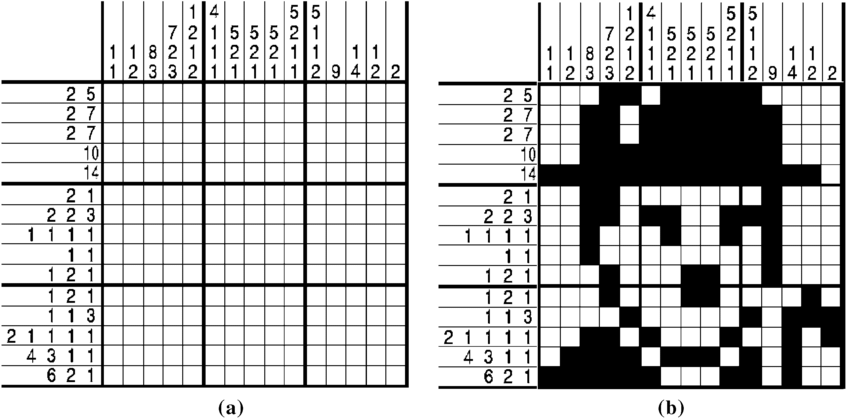
\includegraphics[width=.55\textwidth,align=t]{teaser}
  \end{tabularx}
  \smallskip

  \underline{Tutorial}: Here are some simple $5\times5$ puzzles as a tutorial.
  \smallskip

  \hspace{-15pt} \begin{tabularx}{1.1\linewidth}{c|X|c}
    \multicolumn{3}{l}{Example 1: Complete Row.}\\
    \adjustbox{valign=t}{ \small
      \begin{tabular}{|*5{c|}c}
        \cline{1-5}
        & & & & & 5\\\cline{1-5}
        & & & & & 0\\\cline{1-5}
        & & & & & 0\\\cline{1-5}
        & & & & & 0\\\cline{1-5}
        & & & & & 0\\\cline{1-5}
        \multicolumn{1}{c}{1} & \multicolumn{1}{c}{1} & \multicolumn{1}{c}{1} & \multicolumn{1}{c}{1} & \multicolumn{1}{c}{1} & 
      \end{tabular}}
    &
    {\footnotesize
      a) The grid on the left has zeros in the rows 2, 3, 4 and 5. These rows are empty.\newline
      b) Row 1 contains the value 5. All 5 boxes are to be colored.\newline
      c) This is confirmed by the columns. All columns have 1. Each column has only 1 filled box.}
    &
    \adjustbox{valign=t}{\small  \begin{tabular}{|*5{c|}c}
      \cline{1-5}
      
      \cellcolor{gray} & \cellcolor{gray} & \cellcolor{gray} & \cellcolor{gray} & \cellcolor{gray} & 5\\\cline{1-5}
                       & & & & & 0\\\cline{1-5}
                       & & & & & 0\\\cline{1-5}
                       & & & & & 0\\\cline{1-5}
                       & & & & & 0\\\cline{1-5}
      \multicolumn{1}{c}{1} & \multicolumn{1}{c}{1} & \multicolumn{1}{c}{1} & \multicolumn{1}{c}{1} & \multicolumn{1}{c}{1} & 
    \end{tabular}}

  \\\hline
  \multicolumn{3}{l}{Example 2: Complete Column.}\\
  \adjustbox{valign=t}{ \small
    \begin{tabular}{|*5{c|}c}
      \cline{1-5}
      & & & & & 1\\\cline{1-5}
      & & & & & 1\\\cline{1-5}
      & & & & & 1\\\cline{1-5}
      & & & & & 1\\\cline{1-5}
      & & & & & 1\\\cline{1-5}
      \multicolumn{1}{c}{0} & \multicolumn{1}{c}{0} & \multicolumn{1}{c}{0} & \multicolumn{1}{c}{0} & \multicolumn{1}{c}{5} & 
    \end{tabular}}
  &
  {\footnotesize
    a) The grid on the left has zeros in columns 1, 2, 3 and 4. These columns are empty.\newline
    b) Column 5 contains the value 5. All 5 boxes are to be colored.\newline
    c) This is confirmed by the 1(s) in all the rows. Each row has only 1 filled box.}
  &
  \adjustbox{valign=t}{ \small
    \begin{tabular}{|*5{c|}c}
      \cline{1-5}
      & & & & \cellcolor{gray} & 1\\\cline{1-5}
      & & & & \cellcolor{gray} & 1\\\cline{1-5}
      & & & & \cellcolor{gray} & 1\\\cline{1-5}
      & & & & \cellcolor{gray} & 1\\\cline{1-5}
      & & & & \cellcolor{gray} & 1\\\cline{1-5}
      \multicolumn{1}{c}{0} & \multicolumn{1}{c}{0} & \multicolumn{1}{c}{0} & \multicolumn{1}{c}{0} & \multicolumn{1}{c}{5} & 
    \end{tabular}}

  \\\hline
  \multicolumn{3}{l}{Example 3: Cross.}\\
  \adjustbox{valign=t}{ \small
    \begin{tabular}{|*5{c|}c}
      \cline{1-5}
      & & & & & 1\\\cline{1-5}
      & & & & & 1\\\cline{1-5}
      & & & & & 5\\\cline{1-5}
      & & & & & 1\\\cline{1-5}
      & & & & & 1\\\cline{1-5}
      \multicolumn{1}{c}{1} & \multicolumn{1}{c}{1} & \multicolumn{1}{c}{5} & \multicolumn{1}{c}{1} & \multicolumn{1}{c}{1} & 
    \end{tabular}}
  &
  {\footnotesize

    a) The grid on the left has 1 in columns 1, 2, 4 and 5. There is one filled box in each column.\newline
    b) Rows 1, 2, 4 and 5, each have 1. There is one filled box in each row.\newline
    c) Column 3 and row 3 both have 5. The middle row and middle column is completely filled.}
  &
  \adjustbox{valign=t}{ \small
    \begin{tabular}{|*5{c|}c}
      \cline{1-5}
      & & \cellcolor{gray} & & & 1\\\cline{1-5}
      & & \cellcolor{gray} & & & 1\\\cline{1-5}
      \cellcolor{gray} & \cellcolor{gray} & \cellcolor{gray} & \cellcolor{gray} & \cellcolor{gray} & 5\\\cline{1-5}
      & & \cellcolor{gray} & & & 1\\\cline{1-5}
      & & \cellcolor{gray} & & & 1\\\cline{1-5}
      \multicolumn{1}{c}{1} & \multicolumn{1}{c}{1} & \multicolumn{1}{c}{5} & \multicolumn{1}{c}{1} & \multicolumn{1}{c}{1} & 
    \end{tabular}}
  \\\hline  
\end{tabularx}

\hspace{-15pt} \begin{tabularx}{1.1\linewidth}{c|X|c}
  \multicolumn{3}{l}{Example 4: Empty Square.}\\
  \adjustbox{valign=t}{ \small
    \begin{tabular}{|*5{c|}c}
      \cline{1-5}
      & & & & & 0\\\cline{1-5}
      & & & & & 3\\\cline{1-5}
      & & & & & {\tiny 1,1}\\\cline{1-5}
      & & & & & 3\\\cline{1-5}
      & & & & & 0\\\cline{1-5}
      \multicolumn{1}{c}{0} & \multicolumn{1}{c}{3} & \multicolumn{1}{c}{\tiny 1,1} & \multicolumn{1}{c}{3} & \multicolumn{1}{c}{0} & 
    \end{tabular}}
  &
  {\footnotesize
    a) Two numbers, e.g. 1,1, indicate two boxes in the corresponding row and column, with some space between them.\newline
    b) Rows 1 and 5, and columns 1 and 5 are zero. These are empty.\newline
    c) Row 3 and column 3 are 1,1. There are two boxes, each of length 1, with at least one space between them.}
  &
  \adjustbox{valign=t}{ \small
    \begin{tabular}{|*5{c|}c}
      \cline{1-5}
      & & & & & 0\\\cline{1-5}
      & \cellcolor{gray} & \cellcolor{gray} & \cellcolor{gray} & & 3\\\cline{1-5}
      & \cellcolor{gray} &  & \cellcolor{gray} & & {\tiny 1,1}\\\cline{1-5}
      & \cellcolor{gray} & \cellcolor{gray} & \cellcolor{gray} & & 3\\\cline{1-5}
      & & & & & 0\\\cline{1-5}
      \multicolumn{1}{c}{0} & \multicolumn{1}{c}{3} & \multicolumn{1}{c}{\tiny 1,1} & \multicolumn{1}{c}{3} & \multicolumn{1}{c}{0} & 
    \end{tabular}}

  \\\hline
\end{tabularx}
\smallskip

Here are some interesting examples.
\smallskip

\centerline{\hfill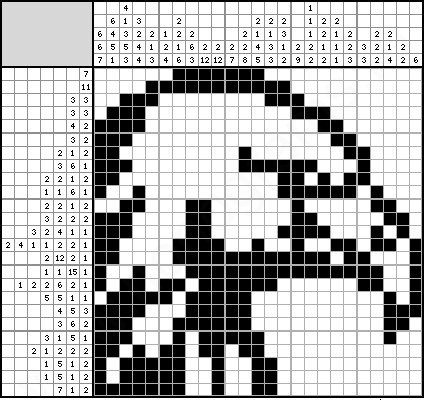
\includegraphics[width=.3\linewidth]{eagle}\hfill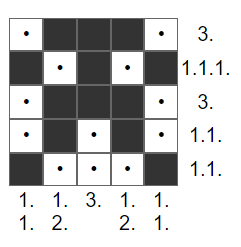
\includegraphics[width=.3\linewidth]{sporg}\hfill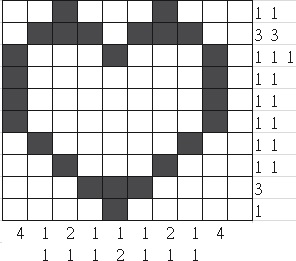
\includegraphics[width=.3\linewidth]{heart}\hfill}

\begin{parts}
  \part In the space below, fill in the cells to solve the five nonograms.. See above to see how to fill a cell.
  \begin{solution}

    \begin{tabularx}{\linewidth}{c|c|c}
      \small
      \begin{tabular}{|*5{c|}c}
        \cline{1-5}
        & \cellcolor{gray} & & \cellcolor{gray} & & {\tiny 1,1}\\\cline{1-5}
        & \cellcolor{gray} & & \cellcolor{gray} & & {\tiny 1,1}\\\cline{1-5}
        & \cellcolor{gray} & \cellcolor{gray} & \cellcolor{gray} & & 3\\\cline{1-5}
        & \cellcolor{gray} & & \cellcolor{gray} & & {\tiny 1,1}\\\cline{1-5}
        & \cellcolor{gray} & & \cellcolor{gray} & & {\tiny 1,1}\\\cline{1-5}
        \multicolumn{1}{c}{0} & \multicolumn{1}{c}{5} & \multicolumn{1}{c}{1} & \multicolumn{1}{c}{5} & \multicolumn{1}{c}{0} & 
      \end{tabular}
      &
      \small
      \begin{tabular}{|*5{c|}c}
        \cline{1-5}
        &  & \cellcolor{gray} &  & & 1\\\cline{1-5}
        & \cellcolor{gray} & & \cellcolor{gray} & & {\tiny 1,1}\\\cline{1-5}
        & \cellcolor{gray} &  & \cellcolor{gray} & & {\tiny 1,1}\\\cline{1-5}
        & \cellcolor{gray} & \cellcolor{gray} & \cellcolor{gray} & & 3\\\cline{1-5}
        & \cellcolor{gray} &  & \cellcolor{gray} & & {\tiny 1,1}\\\cline{1-5}
        \multicolumn{1}{c}{0} & \multicolumn{1}{c}{4} & \multicolumn{1}{c}{\tiny 1,1} & \multicolumn{1}{c}{4} & \multicolumn{1}{c}{0} & 
      \end{tabular}
      &
      \small
      \begin{tabular}{|*5{c|}c}
        \cline{1-5}
        & \cellcolor{gray} & \cellcolor{gray} &  & & 2\\\cline{1-5}
        & \cellcolor{gray} & & \cellcolor{gray} & & {\tiny 1,1}\\\cline{1-5}
        & \cellcolor{gray} & \cellcolor{gray} &  & & 2\\\cline{1-5}
        & \cellcolor{gray} &  & \cellcolor{gray} & & {\tiny 1,1}\\\cline{1-5}
        & \cellcolor{gray} & \cellcolor{gray} &  & & 2\\\cline{1-5}
        \multicolumn{1}{c}{0} & \multicolumn{1}{c}{5} & \multicolumn{1}{c}{\tiny 1,1,1}  & \multicolumn{1}{c}{\tiny 1,1}  & \multicolumn{1}{c}{0} & 
      \end{tabular}  
    \end{tabularx}
    \bigskip

    \hspace{75pt}\begin{tabularx}{\linewidth}{c|c}
      \small
      \begin{tabular}{|*5{c|}c}
        \cline{1-5}
        & \cellcolor{gray} & \cellcolor{gray} & \cellcolor{gray} & & 3\\\cline{1-5}
        &  & \cellcolor{gray} &  & & 1\\\cline{1-5}
        &  & \cellcolor{gray} &  & & 1\\\cline{1-5}
        &  & \cellcolor{gray} &  & & 1\\\cline{1-5}
        & \cellcolor{gray} & \cellcolor{gray} & \cellcolor{gray} & & 3\\\cline{1-5}
        \multicolumn{1}{c}{0} & \multicolumn{1}{c}{\tiny 1,1} & \multicolumn{1}{c}{5} & \multicolumn{1}{c}{\tiny1,1} & \multicolumn{1}{c}{0} & 
      \end{tabular}
      &
      \small
      \begin{tabular}{|*5{c|}c}
        \cline{1-5}
        & \cellcolor{gray} & \cellcolor{gray} &  & & 2\\\cline{1-5}
        & \cellcolor{gray} & & \cellcolor{gray} & & {\tiny 1,1}\\\cline{1-5}
        & \cellcolor{gray} & \cellcolor{gray} &  & & 2\\\cline{1-5}
        & \cellcolor{gray} &  & \cellcolor{gray} & & {\tiny 1,1}\\\cline{1-5}
        & \cellcolor{gray} & \cellcolor{gray} &  & & 2\\\cline{1-5}
        \multicolumn{1}{c}{0} & \multicolumn{1}{c}{5} & \multicolumn{1}{c}{\tiny 1,1,1}  & \multicolumn{1}{c}{\tiny 1,1}  & \multicolumn{1}{c}{0} & 
      \end{tabular}    
    \end{tabularx}
  \end{solution}

  \part What is the hidden message in the above 5 nonograms?
  \begin{solution}
    % Enter your solution here.
    HABIB
  \end{solution}

  \part How many different nonograms can be made from a $5\times5$ grid without any clues? Please explain your answer. (Explaination shouldn't be too long. 1-2 line(s) are sufficient enough.)
  \begin{solution}
    The numbers of nonograms made increases with the exponent of 2 as \(2^n\). Since a 5 x 5 grid has 25 squares the number of possible nanograms would be \(2^{25}\) = 33554432. 
  \end{solution}

  \part How many different nonograms can be made from a $5\times5$ grid with clues? Please explain your answer. (Explaination shouldn't be too long. 1-2 line(s) are sufficient enough.)
  \begin{solution}
    % Enter your solution here.
    When clues are given there can only be one nonogram which satisfies all the clues, hence only 1 nonogram can be made with clues.
  \end{solution}
\end{parts}

\end{questions}

\end{document}

%%% Local Variables:
%%% mode: latex
%%% TeX-master: t
%%% End:
